\newpage
\chapter{Prototypische Implementierung}
Dieses Kapitel widmet sich der Implementierung der zuvor beschriebenen Hardware-Health-Monitoring-Systemarchitektur. Die Umsetzung erfolgt im .NET 4.7-Framework unter Verwendung der Programmiersprache C\#.\\
Zur Orientierung in der Projektstruktur visualisiert Abbildung \ref{fig:Namespaces} die Verzeichnis (Namespace) Aufteilung der Software.  
\begin{center}
    \begin{figure}[h!]
        \centering
        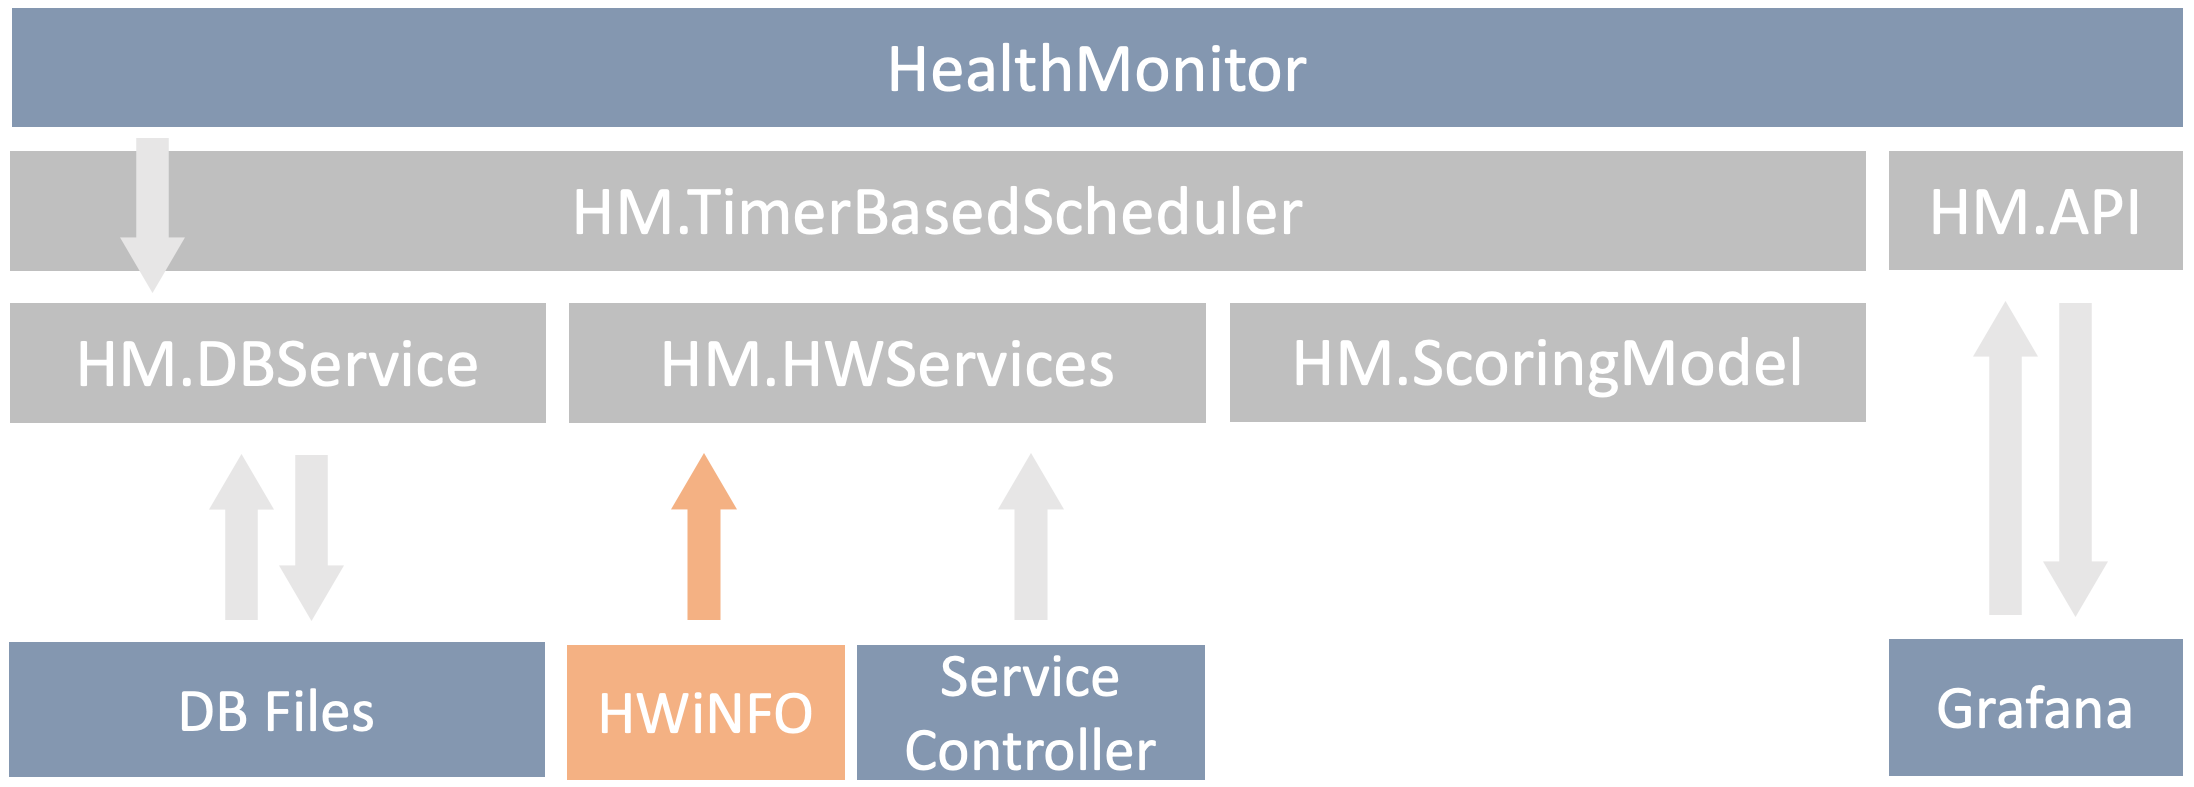
\includegraphics[width=1\textwidth]{Namespaces.png}
        \caption{Verzeichnis Aufteilung des Hardware Health Monitor Programms}
        \label{fig:Namespaces}
    \end{figure}
\end{center}
%\section{HealthMonitor}
%\section{HM.API}
%\section{HM.TimerBasedScheduler}
%\section{HM.HWServices}
%\section{HM.DBServices}
%\section{HM.ScoringModel}
%\section{Aufsetzen des Grafanadashboards}
